\section{The Overshadowed Virgin and the Hill Country of Judea}\label{sec:overshadowed-virgin}

At the close of the Book of Exodus, the moment Moses raises the Tabernacle and draws the veil before the Ark, the cloud of glory covers the sanctuary so completely that even Moses cannot cross the threshold (Exod 40:32--36 [MT/LXX 40:34--38]). From that hour, the cloud by day and fire by night governed every halt and march of Israel across the desert.

Centuries later, in an obscure town of Galilee, the angel Gabriel stands before a young virgin betrothed to a man of the house of David and announces that the same Spirit and power of the Most High will come upon her and overshadow her (Luke 1:26--35). What descended in the wilderness upon acacia wood, linen curtains, and beaten gold now takes human flesh from a woman's own body. The dwelling of God is no longer a portable chest hidden behind a veil; it is a living mother carrying the Son of the Most High. Across the Annunciation, the journey into the hill country of Judah, the greeting of Elizabeth, and the canticle of the \textit{Magnificat}, St.\ Luke unfolds that fulfillment in exact scriptural detail.

\subsection{The Annunciation and the Cloud of Overshadowing (Luke 1:26--38)}

Luke introduces the Annunciation in the sixth month of Elizabeth's pregnancy, setting the scene in sharp contrast to the opening episode of his Gospel. Earlier, Gabriel had appeared to the priest Zechariah beside the golden altar of incense inside the Jerusalem Temple, where Zechariah hesitated before the promise---``Whereby shall I know this? For I am an old man, and my wife is advanced in years'' (Luke 1:18)---and was struck dumb until the child's birth (Luke 1:20). Now the same archangel leaves the precincts of stone and gold and is sent ``from God into a city of Galilee, called Nazareth, to a virgin espoused to a man whose name was Joseph, of the house of David: and the virgin's name was Mary'' (Luke 1:26--27). Before any word is spoken of the conception, Gabriel addresses her with a title that stands in the place of her given name:

\begin{scriptureblock}
And the angel being come in, said unto her: Hail, full of grace, the Lord is with thee: blessed art thou among women. \textnormal{(Luke 1:28)}
\end{scriptureblock}

The Greek participle translated ``full of grace'' (Latin \textit{gratia plena}) is \textit{kecharitomene}, the perfect passive participle of \textit{charitoo}. Across the entire New Testament, the verb \textit{charitoo} occurs only twice: here in Gabriel's salutation at Luke 1:28, and in St.\ Paul's opening hymn of blessing in Ephesians 1:6, ``Unto the praise of the glory of his grace, in which he hath graced us, in his beloved son.'' The perfect tense expresses a divine action already accomplished whose effect abides in the present. Before Gabriel discloses what God is about to work within her, Mary stands already transformed by favor---an enduring state that the angel echoes two verses later: ``Fear not, Mary, for thou hast found grace with God'' (Luke 1:30). In the Greek textual tradition, the closing clause ``blessed art thou among women'' stands at Luke 1:28 in the Byzantine Greek manuscript tradition and in St.\ Jerome's Vulgate, while the Alexandrian critical text omits it in Gabriel's greeting; every manuscript preserves it on Elizabeth's lips fourteen verses later, joined directly to ``the fruit of thy womb'' (Luke 1:42).

Gabriel then proclaims the royal promise of the house of David: the child conceived in her womb will be named Jesus, ``He shall be great and shall be called the Son of the Most High. And the Lord God shall give unto him the throne of David his father: and he shall reign in the house of Jacob for ever. And of his kingdom there shall be no end'' (Luke 1:32--33). Unlike Zechariah, Mary asks for no authenticating sign; she asks only how this birth will come to pass without violating her state of life: ``How shall this be done, because I know not man?'' (Luke 1:34). Because she is already betrothed to Joseph, the question presupposes a settled resolve to remain a virgin. Gabriel answers by announcing a direct creative act of God:

\begin{scriptureblock}
And the angel answering, said to her: The Holy Ghost shall come upon thee and the power of the Most High shall overshadow thee. And therefore also the Holy which shall be born of thee shall be called the Son of God. \textnormal{(Luke 1:35)}
\end{scriptureblock}

In Greek, Gabriel's promise reads \textit{Pneuma hagion epeleusetai epi se, kai dynamis Hypsistou episkiasei soi}; in Latin, \textit{Spiritus Sanctus superveniet in te, et virtus Altissimi obumbrabit tibi}. The verb \textit{episkiazo}, ``to overshadow,'' unites a select group of New Testament theophanies. Across the entire New Testament, \textit{episkiazo} occurs exactly five times. Four of the five describe a direct manifestation of divine glory revealing the Son of God: here at the Annunciation (Luke 1:35), and in all three Synoptic accounts of the Transfiguration, where a bright cloud descends upon the mountain and overshadows the disciples while the Father's voice proclaims, ``This is my beloved Son, in whom I am well pleased: hear ye him'' (Matt 17:5; Mark 9:7, numbered 9:6 in the Vulgate; Luke 9:34, ``there came a cloud and overshadowed them''). The fifth occurrence stands in Luke's second volume, where the sick are carried into the streets of Jerusalem ``that, when Peter came, his shadow at the least might overshadow any of them and they might be delivered from their infirmities'' (Acts 5:15)---a derivative sign of healing flowing from the Spirit of the risen Lord active in the apostolic Church.

In the Greek Old Testament, that same verb belongs to the cloud of glory resting upon the wilderness sanctuary. In Brenton's English rendering of the Septuagint, Exodus 40:35 states that Moses could not enter the tabernacle of testimony ``because the cloud overshadowed it, and the tabernacle was filled with the glory of the Lord.'' The Book of Numbers repeats the idiom throughout Israel's marches: the cloud ``overshadows the tabernacle'' while the camp rests (Num 9:18, 20, 22) and ``overshadowed them by day, when they departed from the camp'' (Num 10:36 in the Septuagint verse order). In the same Greek translation, the golden cherubim stretch out their wings above the Ark, ``overshadowing the propitiatory with their wings'' (Exod 25:20; 38:8 in the Septuagint; cf.\ 1 Chr 28:18).

Comparing the Greek and Latin Bibles reveals a precise textual channel. In Exodus 40:32--33, St.\ Jerome did not translate with \textit{obumbro}; he wrote \textit{operuit}, \textit{operiente}, and \textit{operuerat} (``covered'' and ``covering''). The verbal link between Exodus 40 and Luke 1:35 therefore passes through the Greek Septuagint rather than through the Latin text of Exodus. Yet Jerome's \textit{obumbro} opens a rich Latin echo of its own: the Book of Wisdom recalls the Exodus cloud with \textit{nubes castra eorum obumbrabat}, ``For a cloud overshadowed their camps'' (Wis 19:7), and the Epistle to the Hebrews describes ``the cherubims of glory overshadowing the propitiatory'' (\textit{cherubim gloriae obumbrantia propitiatorium}, Heb 9:5), rendering the Greek compound \textit{kataskiazo}, which appears nowhere else in the New Testament.

Even closer is the exact verbal convergence in the Greek and Latin Psalter. In Psalm 90(91):4, the Septuagint reads \textit{en tois metaphrenois autou episkiasei soi, kai hypo tas pterygas autou elpieis}, matching the Latin Vulgate \textit{Scapulis suis obumbrabit tibi, et sub pennis ejus sperabis} and the Douay-Rheims rendering: ``He will overshadow thee with his shoulders: and under his wings thou shalt trust.'' Both the inflected Greek phrase \textit{episkiasei soi} and the inflected Latin phrase \textit{obumbrabit tibi} match Gabriel's words to Mary syllable for syllable, and the psalm immediately pairs that overshadowing with refuge ``under his wings'' (\textit{hypo tas pterygas autou})---the exact posture of the Ark resting beneath the outspread wings of the cherubim in the inner oracle of Solomon's Temple (1 Kgs 8:6, where the Septuagint likewise reads \textit{hypo tas pterygas ton cheroubein}). A second psalm deepens the echo: in Psalm 139(140):8, the anointed king prays, ``O Lord, Lord, the strength of my salvation: thou hast overshadowed my head in the day of battle''---in Greek \textit{dynamis tes soterias mou, epeskiasas}, and in Latin \textit{virtus salutis meae, obumbrasti}, joining ``power'' (\textit{dynamis} / \textit{virtus}) directly to the verb of overshadowing just as Gabriel does at Nazareth.

A reflection on the image of shadow transmitted under St.\ Gregory of Nyssa's name in St.\ Thomas Aquinas's \textit{Catena Aurea on Luke} 1:35 observes: ``Or he says, \textit{overshadow thee}, because as a shadow takes its shape from the character of those bodies which go before it, so the signs of the Son's Deity will appear from the power of the Father.'' To this the Venerable Bede adds the cooling purity of that cloud in the same \textit{Catena Aurea} entry on Luke 1:35: ``There shall be no flame of desire in thee when the Holy Spirit shall overshadow thee.'' Gathering the patristic tradition on \textit{obumbrabit tibi}, Cornelius a Lapide states both the hidden veil and the creative work accomplished beneath it:

\begin{quote}\small
But more simply, the meaning is, It will cover thee as with a veil, i.e., will secretly work a mighty operation in thee; for it will be such and so great a one that no man or angel can penetrate into or comprehend it. For, first, it will form in thee the perfect humanity of Christ; and, secondly, it will unite the same in a certain ineffable manner to the Person of the Word.
\end{quote}

God does not force His entry into the living sanctuary. Gabriel offers Mary the sign of her aged kinswoman Elizabeth, already in her sixth month, ``Because no word shall be impossible with God'' (Luke 1:36--37), and waits for her free reply: ``And Mary said: Behold the handmaid of the Lord: be it done to me according to thy word. And the angel departed from her'' (Luke 1:38). Contemplating that suspended instant in his fourth homily \textit{Super Missus est} (IV.8), St.\ Bernard of Clairvaux speaks to the Virgin on behalf of the entire waiting race of Adam:

\begin{quote}\small
The angel awaits your reply, for it is time that he should return to God, Who sent him. We, too, are waiting, O Lady, for a word of mercy---we, who are groaning under the sentence of condemnation. See, the price of our salvation is offered to you; if you consent, we shall at once be delivered. By the Eternal Word of God we were all created, and behold we die. By your short answer we shall be refreshed and recalled to life. ... Answer, then, quickly to the angel---yes, through the angel give your consent to your God. Answer the word, receive the Word. Utter yours, conceive the Divine. ... Open, O Blessed Virgin, your heart to faith, your lips to compliance, your bosom to your Creator.
\end{quote}

\ifdefined\TriptychPrintEdition
\Needspace{34\baselineskip}
\begin{center}
\begin{tikzpicture}
  \node[anchor=south west, inner sep=0] (platevi) at (0,0)
    {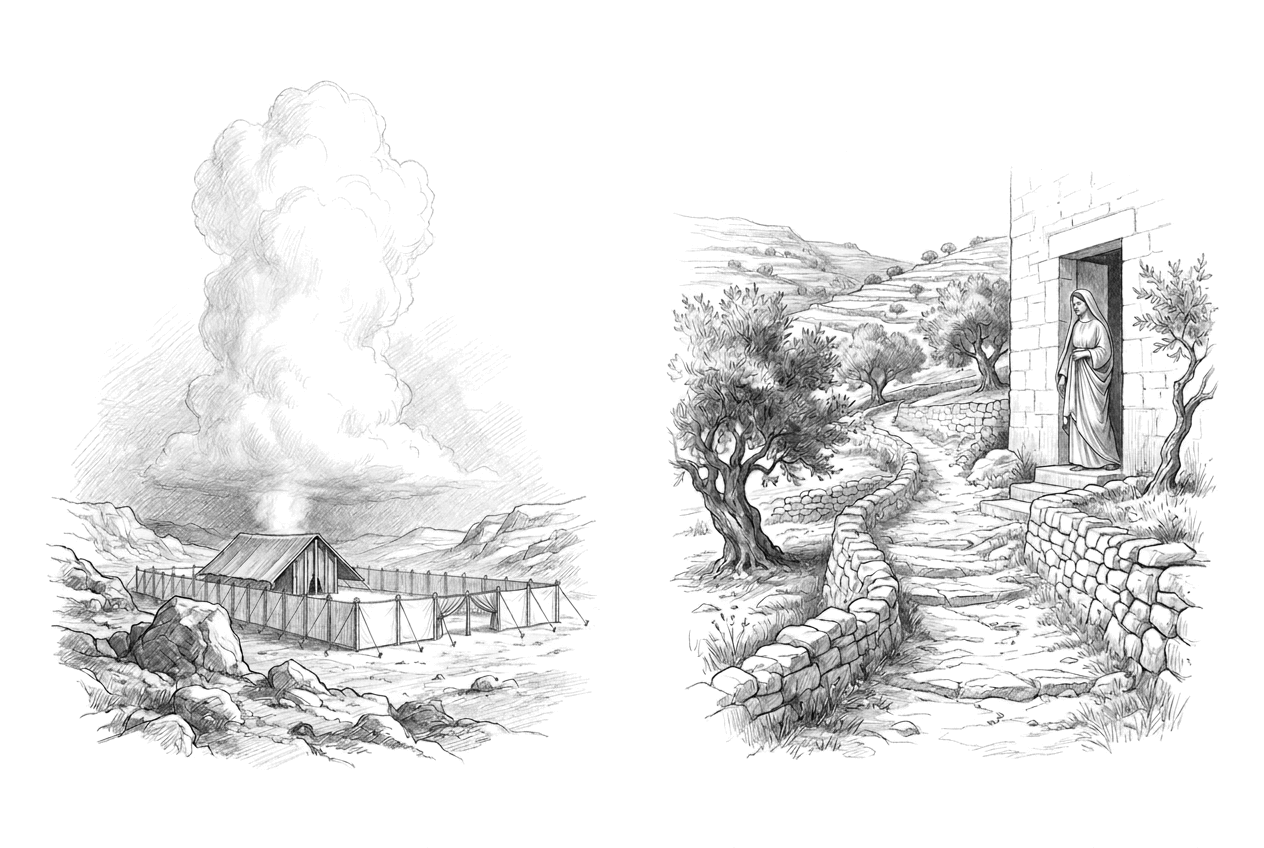
\includegraphics[width=0.94\linewidth]{theology/mariology/ark-of-the-covenant/artwork/visitation-ark-typology-graphite.png}};
  \begin{scope}[x={(platevi.south east)}, y={(platevi.north west)}]
    \node[font=\scriptsize, align=center, anchor=center, inner sep=1pt] at (0.25, 0.03)
      {\textit{The Cloud Overshadowing the Tent}\\(Exod 40:34--35)};
    \node[font=\scriptsize, align=center, anchor=center, inner sep=1pt] at (0.75, 0.03)
      {\textit{The Living Ark in the Hill Country of Judea}\\(Luke 1:35, 39--45)};
  \end{scope}
\end{tikzpicture}
\end{center}\nopagebreak[4]
\else
\begin{studybox}{Plate VI: From the Overshadowed Tabernacle to the Hill Country of Judea}
\textbf{Left panel (\textit{The Cloud Overshadowing the Tent}, Exod 40:34--35):} In a rocky wilderness valley framed by desert ridges, the rectangular curtained courtyard of the Tabernacle encloses the pitched Tent of Meeting. Above the sanctuary rises a towering, luminous pillar of cloud whose base descends directly onto the tent roof, expressing the glory of the Lord filling the dwelling place so fully that Moses cannot enter.

\textbf{Right panel (\textit{The Living Ark in the Hill Country of Judea}, Luke 1:35, 39--45):} A stepped stone path winds between dry-laid terrace walls and gnarled olive trees across the terraced slopes of Judah toward the open threshold of a quiet limestone dwelling. Framed in the doorway stands the veiled Virgin Mary, serene and recollected, bearing the Incarnate Word into the priestly household of Zechariah and Elizabeth.
\end{studybox}
\fi
\begin{platecaption}
\textbf{Plate VI.} \textit{From the Cloud Over the Tent to the Hill Country of Judea.} The wilderness Tabernacle overshadowed by the pillar of cloud (Exod 40:32--33 Douay-Rheims; 40:34--35 MT/LXX) stands beside the Virgin Mary arriving in the terraced hills of Judah after the overshadowing of the Holy Spirit (Luke 1:35, 39--45). The visual pairing expresses the scriptural correspondence between God's indwelling glory in the desert tent and His incarnate presence in the Mother of the Lord; Luke leaves Zechariah's Judean town unnamed, and no identity of exact village site with Kiriath-jearim is implied.
\end{platecaption}

\subsection{The Visitation Beside David's Procession of the Ark (Luke 1:39--56)}

Immediately upon conceiving the Word, Mary sets out southward from Nazareth into the hill country of Judah. Placed beside King David's solemn translation of the Ark of the Covenant out of the Judean hills toward Jerusalem (2 Samuel 6; 1 Chronicles 13--16), Luke's account of the Visitation unfolds a sustained sequence of correspondences. Reading the Greek and Latin texts closely shows that one correspondence turns on a Greek verb unique to Luke across the entire New Testament, others share a close syntactic cadence or an identical span of months, and another pairs two scenes of Spirit-awakened bodily joy expressed through distinct verbs.

\subsubsection{Arising and Going into the Hill Country of Judah (Luke 1:39; 2 Sam 6:2)}

Luke opens the Visitation with swift movement: ``And Mary rising up in those days, went into the hill country with haste into a city of Juda. And she entered into the house of Zachary and saluted Elizabeth'' (Luke 1:39--40). In Greek, \textit{Anastasa de Mariam en tais hemerais tautais eporeuthe eis ten oreinen meta spoudes eis polin Iouda}; in Latin, \textit{Exsurgens autem Maria in diebus illis, abiit in montana cum festinatione, in civitatem Juda}.

David's expedition to retrieve the Ark begins with the same Semitic opening idiom directed into the same highland territory: ``And David arose and went, with all the people that were with him of the men of Juda to fetch the ark of God, upon which the name of the Lord of Hosts is invoked, who sitteth over it upon the cherubims'' (2 Sam 6:2; Latin \textit{Surrexitque David, et abiit, et universus populus qui erat cum eo de viris Juda}). A textual variation in 2 Samuel 6:2 clarifies the geography: the Hebrew consonants \textit{baale yehudah} can be read either as a place name---``from Baale of Judah,'' the older name of Kiriath-jearim in the western Judean hills (compare 1 Chr 13:6, ``the hill of Cariathiarim which is in Juda''), as rendered in the Revised Version and World English Bible---or as ``the men'' or ``rulers'' of Judah, which underlies St.\ Jerome's \textit{de viris Juda} and Brenton's Septuagint ``some of the rulers of Juda.'' Luke leaves Zechariah's town unnamed, calling it simply ``a city of Juda.'' Ancient Christian tradition identifies that town with Ein Karem, nestled in the western hills just outside Jerusalem, along the same Judean ridge that once held Kiriath-jearim and the house of Obed-edom.

In his \textit{Exposition of the Gospel of Luke} (II.19), St.\ Ambrose ponders Mary's haste up into the mountains. She did not hurry out of unbelief in the oracle, nor from uncertainty about the messenger, nor from doubt about the sign, ``but glad for her vow, dutiful in service, hastening for joy, she went into the hill country'' (\textit{quasi laeta pro voto, religiosa pro officio, festina pro gaudio in montana perrexit}). Then Ambrose asks: ``For where else should she, already full of God, hasten but to the heights? The grace of the Holy Spirit knows no slow delays'' (\textit{quo enim iam Deo plena nisi ad superiora cum festinatione contenderet? nescit tarda molimina sancti Spiritus gratia}).

\subsubsection{Elizabeth's Liturgical Outcry (Luke 1:42; 1 Chronicles 15--16)}

The moment Mary's greeting reaches Elizabeth's ears, the Holy Spirit fills the aged kinswoman, and Luke chooses a singular verb to describe her response:

\begin{scriptureblock}
And it came to pass that when Elizabeth heard the salutation of Mary, the infant leaped in her womb. And Elizabeth was filled with the Holy Ghost. And she cried out with a loud voice and said: Blessed art thou among women and blessed is the fruit of thy womb. \textnormal{(Luke 1:41--42)}
\end{scriptureblock}

The Greek verb for ``cried out,'' \textit{anaphoneo} (inflected \textit{anephonesen}), occurs nowhere else in the entire New Testament---a word used only once among all 137,554 words of the Greek New Testament. Its accompanying noun shows a minor manuscript variation: the Alexandrian critical text reads \textit{krauge megale} (``with a loud cry''), whereas the Byzantine Greek tradition reads \textit{phone megale} (``with a loud voice''), matching St.\ Jerome's \textit{voce magna} and the Douay-Rheims wording.

In the Greek Old Testament, that liturgical vocabulary of lifting up a solemn vocal and musical proclamation belongs characteristically to the Levites ministering before the Ark of the Covenant in 1 and 2 Chronicles. After David's first attempt to move the Ark on a cart ended in the death of Uzzah, the king learned from the Law that ``no one ought to carry the ark of God, but the Levites'' (1 Chr 15:2) and summoned the consecrated sons of Levi to bear it ``upon their shoulders, with the staves'' (1 Chr 15:15) amid trumpets, cymbals, psalteries, harps, and sacrifices (1 Chr 15:16, 26--28; 2 Sam 6:12--15). Standard Septuagint lexica note that Greek \textit{anaphoneo} concentrates in those Ark-procession and Temple-dedication verses (1 Chr 15:28; 16:4, 5, 42; 2 Chr 5:13). Brenton's English translation of the Septuagint preserves this recurring sanctuary voice vividly: David bids the Levitical chiefs appoint singers ``to sound aloud with a voice of joy'' (1 Chr 15:16); Israel brings up the Ark ``with shouting ... playing loudly on lutes and harps'' (1 Chr 15:28); David stations Levites before the Ark ``to minister and lift up the voice, and to give thanks and praise the Lord God of Israel'' (1 Chr 16:4, where the Vulgate instead translates \textit{recordarentur}, ``to remember''); trumpets and cymbals stand ready ``to sound aloud'' (1 Chr 16:42); and at Solomon's dedication of the Temple, the singers unite ``in the loud utterance with one voice to give thanks and praise the Lord'' (2 Chr 5:13). Elizabeth, herself ``of the daughters of Aaron'' (Luke 1:5) standing in the household of a serving priest, lifts up the Levitical cry of the sanctuary before the living Ark.

Her words crown that acclamation: ``Blessed art thou among women and blessed is the fruit of thy womb.'' Earlier in Israel's story, Deborah praised Jael---``Blessed among women be Jahel'' (Judg 5:24)---and Ozias praised Judith---``Blessed art thou, O daughter, by the Lord the most high God, above all women upon the earth'' (Jdt 13:23)---because through each woman God struck down an oppressor of His people. Elizabeth now speaks the definitive blessing, disclosing its source in the same breath: Mary is blessed among all women because of the blessed fruit resting within her womb.

\subsubsection{The Question of Reverent Awe (Luke 1:43; 2 Samuel 6:9)}

Immediately after blessing Mary and her child, Elizabeth asks a question whose cadence mirrors King David's cry on the road from Kiriath-jearim:

\begin{scriptureblock}
And David was afraid of the Lord that day, saying: How shall the ark of the Lord come to me? \textnormal{(2 Sam 6:9)}
\end{scriptureblock}

\begin{scriptureblock}
And whence is this to me that the mother of my Lord should come to me? \textnormal{(Luke 1:43)}
\end{scriptureblock}

In their Greek and Latin wording, the two sentences use different interrogatives and different verbs: David asks \textit{Quomodo ingredietur ad me arca Domini?} (``How shall the ark of the Lord enter in to me?''; compare 1 Chr 13:12, ``How can I bring in the ark of God to me?''), whereas Elizabeth asks \textit{Et unde hoc mihi, ut veniat mater Domini mei ad me?} (Greek \textit{kai pothen moi touto hina elthe he meter tou kyriou mou pros eme?}). Yet the parallel structure is plain: both express startled awe and unworthiness at the arrival of God's dwelling at one's own threshold, with ``the mother of my Lord'' occupying the exact structural place once held by ``the ark of the Lord.''

The contrast in tone marks the passage from Sinai to the Gospel. David spoke his question in dread after Uzzah had fallen dead beside the cart on the threshing floor of Nachon; fearful of the Ark's consuming holiness, the king refused to receive it into his own city. Elizabeth speaks her question in the overflowing joy of the Holy Spirit: the same Lord who struck Uzzah at the threshing floor now enters Zechariah's house hidden beneath the heart of His mother, bringing not terror but sanctification.

Cornelius a Lapide, expounding Luke 1:43, draws out the full Christological weight of Elizabeth's words ``the mother of my Lord'':

\begin{quote}\small
Lord, that is God, Who is called absolutely the Lord, because He is King of kings and Lord of lords. Hence it is clear---1.\ That the humanity of Christ was already in Christ endowed with life and united to the Word or Son of God. 2.\ That the Blessed Virgin is rightly called \textit{Theotokos}, i.e., Mother of God and not only \textit{Christotokos}, Mother of Christ, as Nestorius maintained.
\end{quote}

\subsubsection{The Unborn Precursor Leaping Before the Lord (Luke 1:41, 44; 2 Sam 6:14--16)}

Elizabeth explains her astonishment by pointing to what has just happened within her own body: ``For behold as soon as the voice of thy salutation sounded in my ears, the infant in my womb leaped for joy'' (Luke 1:44).

Luke describes the unborn John's movement with the Greek verb \textit{skirtao} (inflected \textit{eskirtesen} in both Luke 1:41 and 1:44; Latin \textit{exsultavit}). Across the entire New Testament, \textit{skirtao} appears exactly three times, all in Luke: twice here at the Visitation (Luke 1:41, 44) and once in the Beatitudes (Luke 6:23, ``Be glad in that day and rejoice,'' literally ``leap''). In the Greek Old Testament, \textit{skirtao} connects directly to two celebrated passages: in Genesis 25:22 (Brenton's Septuagint), ``the babes leaped within her'' as Rebekah carried Jacob and Esau, and in the Exodus hymn of Psalm 113(114):4, 6 (Swete Greek \textit{ta ore eskirtesan hos krioi}, Latin \textit{Montes exsultaverunt ut arietes}), ``The mountains skipped like rams, and the hills like the lambs of the flock'' at the presence of the Lord leading Israel out of Egypt (compare also Mal 3:20 in Brenton's Septuagint, where those who fear the Lord's name ``bound as young calves let loose from bonds'').

By contrast, 2 Samuel 6:14 and 6:16 do not use \textit{skirtao}. In the Clementine Vulgate and Douay-Rheims, David ``danced with all his might before the Lord'' (\textit{saltabat}, 6:14) and Michal watches him ``leaping and dancing before the Lord'' (\textit{subsilientem atque saltantem}, 6:16); in Brenton's Septuagint, verse 14 states that David ``sounded with well-tuned instruments before the Lord'' and verse 16 that he was ``dancing and playing.'' The correspondence between David dancing before the Ark and the unborn John leaping before Mary is therefore a narrative and theological parallel of Spirit-awakened bodily exultation before the approaching Lord, not a shared Greek verb.

The Fathers recognized in John's leap the first prophetic act of the Baptist's ministry, awakened by the presence of the Incarnate Lord within Mary. In his \textit{Exposition of the Gospel of Luke} (II.23), St.\ Ambrose observes the order of grace in the encounter:

\begin{quote}\small
Elizabeth heard the voice first, but John perceived the grace first; she heard by the order of nature, he leaped by reason of the mystery; she perceived the coming of Mary, he the coming of the Lord. ... The infant leaped, the mother was filled. ... And the one is filled after conceiving, the other before conceiving.
\end{quote}

In Ambrose's crisp Latin (\textit{Vocem prior Elizabeth audivit, sed Joannes prior gratiam sensit: illa naturae ordine audivit, iste exsultavit ratione mysterii: illa Mariae, iste Domini sensit adventum}), Mary's voice is the instrument through which the invisible Lord sanctifies His precursor in the womb; two paragraphs later Ambrose exclaims, ``I perceive a miracle, I recognize a mystery: the mother of the Lord is pregnant with the Word, full of God'' (\textit{Miraculum sentio, cognosco mysterium: mater Domini Verbo foeta, Deo plena est}, II.25). Earlier in the fourth century, St.\ Athanasius of Alexandria had cited the same moment in his \textit{Oration III against the Arians} (33) to prove the real presence of the divine Word in Mary's womb: ``Many for instance have been made holy and clean from all sin; nay, Jeremiah was hallowed even from the womb, and John, while yet in the womb, leapt for joy at the voice of Mary Bearer of God.''

\subsubsection{Three Months of Household Blessing (Luke 1:56; 2 Sam 6:11; 1 Chr 13:14)}

After Mary sings the \textit{Magnificat}, Luke closes the Visitation with a single quiet sentence of time and departure: ``And Mary abode with her about three months. And she returned to her own house'' (Luke 1:56; Greek \textit{Emeinen de Mariam syn aute hos menas treis}, with \textit{hosei} in the Byzantine Greek tradition; Latin \textit{Mansit autem Maria cum illa quasi mensibus tribus}).

That exact span of three months stands at the turning point of David's translation of the Ark. After the shock of Uzzah's death, David turns the Ark aside into the house of Obed-edom the Gethite: ``And the ark of the Lord abode in the house of Obededom the Gethite three months: and the Lord blessed Obededom, and all his household'' (2 Sam 6:11). The Chronicler repeats the notice in Latin phrasing that converges word for word with Luke 1:56: \textit{Mansit ergo arca Dei in domo Obededom tribus mensibus}, ``And the ark of God remained in the house of Obededom three months: and the Lord blessed his house, and all that he had'' (1 Chr 13:14).

In Obed-edom's house, those three months turned fear into gladness: the visible blessing resting on his household convinced David that the Ark could be brought up to Zion with joy, sacrifice, and song (2 Sam 6:12--15). In the priestly house of Zechariah and Elizabeth, Mary's three-month stay fills the home with the silent work of sanctification until the birth of John and the unloosing of Zechariah's prophetic canticle, the \textit{Benedictus} (Luke 1:57--79). St.\ Ambrose (\textit{Exposition of the Gospel of Luke} II.29) dwells on that mystical duration:

\begin{quote}\small
Rightly is holy Mary introduced both as having fulfilled an office of charity and as having observed a mystical number. For familiarity alone is not the reason she remained so long, but also the advancement of so great a prophet. For if at her first entrance such great progress occurred, that at Mary's salutation the infant leaped in the womb and the mother of the infant was filled with the Holy Spirit, how much do we think the presence of holy Mary added through the intimacy of so long a time?
\end{quote}

\subsection{The Magnificat: The Sanctuary Redirecting All Praise to God (Luke 1:46--55)}

Elizabeth concludes her greeting by crowning Mary's faith: ``And blessed art thou that hast believed, because those things shall be accomplished that were spoken to thee by the Lord'' (Luke 1:45). Mary replies neither by denying the wonder worked in her nor by letting praise come to rest upon herself. Like the golden Ark that exists solely to bear the Word of the covenant and direct every eye to the glory dwelling above the mercy seat, she turns every word of praise immediately upward to God:

\begin{scriptureblock}
And Mary said: My soul doth magnify the Lord. And my spirit hath rejoiced in God my Saviour. Because he hath regarded the humility of his handmaid: for behold from henceforth all generations shall call me blessed. Because he that is mighty hath done great things to me: and holy is his name. \textnormal{(Luke 1:46--49)}
\end{scriptureblock}

Her opening verses echo Hannah's song of thanksgiving at Shiloh, the sanctuary where the Ark of God stood before the young Samuel (1 Sam 1:9; 3:3): ``My heart hath rejoiced in the Lord, and my horn is exalted in my God'' (1 Sam 2:1). Where Hannah sang before the tent of Shiloh over the birth of the prophet who would anoint David, Mary sings as the living sanctuary herself over the coming of David's eternal Son. Even as she prophesies that ``all generations shall call me blessed,'' she states the reason in the very next clause: ``Because he that is mighty hath done great things to me: and holy is his name.'' Her canticle celebrates God's mercy ``from generation unto generations, to them that fear him,'' His mighty arm scattering the proud and raising up the lowly, and His faithful remembrance of what ``he spoke to our fathers: to Abraham and to his seed for ever'' (Luke 1:50--55).

Commenting on Luke 1:46, Cornelius a Lapide preserves a short, luminous saying of St.\ Bernard of Clairvaux (from his sermon on the twelfth chapter of Revelation) on the humility of the \textit{Magnificat}:

\begin{quote}\small
Truly this is a song of high praise, but also of devout humility which suffers her not to retain anything for herself, but gives all back rather to Him Whose blessings bestowed upon herself she was celebrating. Thou, she says, magnifiest the Mother of the Lord, but my soul doth magnify the Lord.
\end{quote}

Because Mary magnifies the Lord without withholding anything for herself, her canticle becomes the pattern of every believing soul and of the whole Church. In his \textit{Exposition of the Gospel of Luke} (II.26), St.\ Ambrose accordingly prays that Mary's soul may be in each believer to magnify the Lord and her spirit in each to exult in God, since every spotless soul receives the Word of God by faith.
